% \chapter{Luồng hoạt động và kiến trúc công cụ}
\chapter{Thiết kế và cài đặt công cụ}
\label{chap:design}

Chương 3 trình bày về quy trình phân tích mã nguồn cho ngôn ngữ Rust bao gồm việc xây dựng cây AST và ánh xạ từ cây AST sang đồ thị CPG.
Chương cũng sẽ đi sâu vào kiến trúc, các thành phần và cài đặt của công cụ.
% Tiếp theo, các thể loại cú pháp Rust sẽ được phân tích để minh họa cách ánh xạ từ cây AST sang đồ thị CPG một cách hiệu quả.
% Ngoài ra, chương cũng sẽ trình bày về các hạn chế hiện thời, nhằm làm rõ các thách thức và định hướng cải tiến công cụ trong tương lai.
Ngoài ra, các thể loại cú pháp Rust sẽ được phân tích để minh họa cách ánh xạ từ cây AST sang đồ thị CPG một cách hiệu quả.

% Nội dung của chương 4 là về việc chuyển đổi mã nguồn sang đồ thị CPG trên các thể loại cú pháp Rust.
% Mức độ cài đặt của công cụ cho việc bao phủ các loại nút AST và ánh xạ chúng sang nút CPG tương ứng sẽ được thảo luận.
% Ngoài ra, chương cũng sẽ trình bày về các hạn chế hiện thời của công cụ.

% \section{Luồng hoạt động}
\section{Luồng hoạt động và cài đặt công cụ}

\begin{figure}[H]
	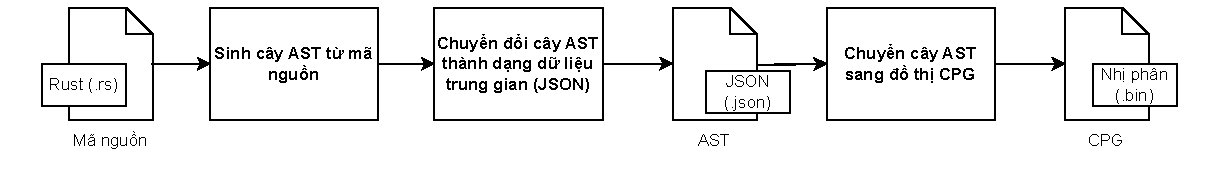
\includegraphics[width=1\columnwidth]{figures/c3/c3_flow_2.drawio.pdf}
	\centering
	\caption{Quy trình phân tích mã nguồn Rust.}
	\label{img:c3_flow_2}
\end{figure}

% \begin{figure}[H]
% 	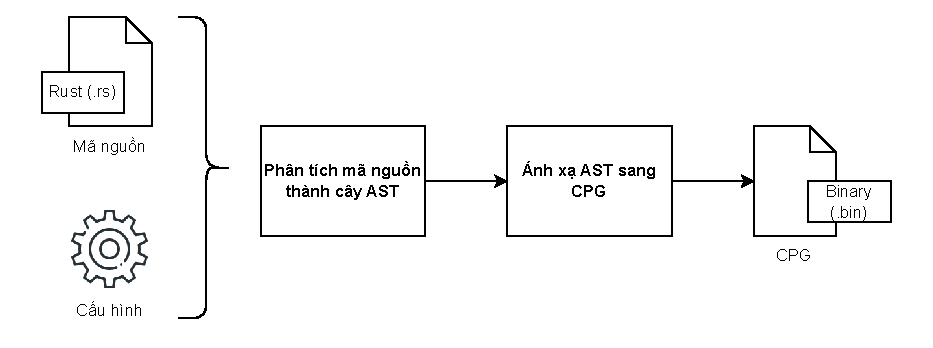
\includegraphics[width=1\columnwidth]{figures/c3/c3_flow.drawio.pdf}
% 	\centering
% 	\caption{Quy trình phân tích mã nguồn Rust.}
% 	\label{img:c3_flow}
% \end{figure}

% \begin{figure}[H]
% 	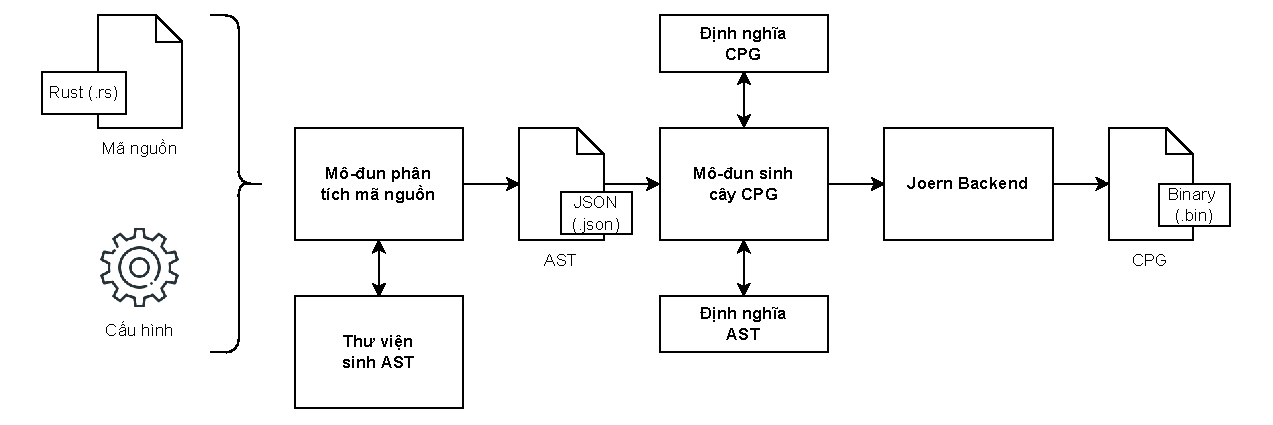
\includegraphics[width=1\columnwidth]{figures/c4/c4_install_flow.drawio.pdf}
% 	\centering
% 	\caption{Kiến trúc công cụ.}
% 	\label{img:c4_install_flow}
% \end{figure}

% \begin{figure}[H]
% 	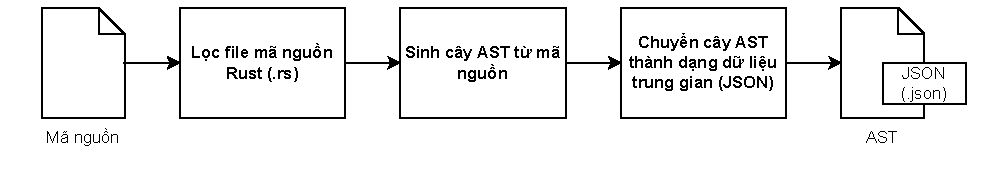
\includegraphics[width=1\columnwidth]{figures/c3/c3_flow_ast.drawio.pdf}
% 	\centering
% 	\caption{Quy trình xây dựng cây AST.}
% 	\label{img:c3_flow_ast}
% \end{figure}

Mục tiêu của công cụ là phân tích mã nguồn Rust và xây dựng đồ thị CPG biểu diễn mã nguồn đó.
% Đầu vào của công cụ là các tệp mã nguồn Rust, đầu ra là đồ thị CPG lưu dưới dạng nhị phân.
Đầu vào của công cụ là các tệp mã nguồn Rust, trong khi đầu ra là đồ thị CPG được lưu dưới dạng nhị phân để dễ dàng xử lý và lưu trữ.
Đồ thị CPG được phục vụ cho việc thực hiện các câu lệnh truy vấn trên đồ thị hoặc quét đồ thị để tìm lỗ hổng trong mã nguồn.
% Với yêu cầu đầu vào, đầu ra như trên, luồng hoạt động của công cụ bao gồm các bước được thể hiện trong hình \ref{img:c3_flow_2}.
Với yêu cầu đầu vào và đầu ra như trên, luồng hoạt động của công cụ được thiết kế thành các bước liên kết chặt chẽ và được thể hiện trong hình \ref{img:c3_flow_2}.
% Chi tiết các bước được tiến hành như sau:
% Các bước này bao gồm phân tích cú pháp mã nguồn, xây dựng cây AST, ánh xạ cây AST sang đồ thị CPG, và cuối cùng là xuất đồ thị dưới định dạng nhị phân.
Chi tiết các bước được tiến hành như sau:

\begin{enumerate}
	\item Từ thư mục của dự án, lọc lấy các tệp mã nguồn Rust (các tệp có đuôi \texttt{.rs}).
	\item Với mỗi tệp mã nguồn, sử dụng thư viện \textit{syn} \cite{synRust} để sinh cây AST từ nội dung mã nguồn của tệp đó.
	\textit{syn} là một thư viện phân tích mã nguồn thành cây AST được sử dụng rộng rãi với nhiều mục đích, trong đó bao gồm việc cài đặt tính năng Procedural Macro \cite{rustlangProceduralMacros} của Rust.
	Tính tới thời điểm hiện tại Rust không có đặc tả ngôn ngữ chính thức, do đó cộng đồng sử dụng Rust Reference \cite{rustReference} coi như phiên bản sát nhất so với một đặc tả ngôn ngữ.
	Thư viện syn xây dựng định nghĩa các nút của cây AST tuân theo Rust Reference.
	\item Chuyển đổi cây AST từ ngôn ngữ Rust sang định dạng JSON.
	Joern có thể được sử dụng cho nhiều ngôn ngữ và Joern Frontend không phụ thuộc vào bộ phân tích ngôn ngữ của một ngôn ngữ nhất định, do vậy cần có định dạng dữ liệu trung gian để chuyển đổi cây AST của bộ phân tích ngôn ngữ sang ngôn ngữ Scala của Joern Frontend.
	Có các kiểu dữ liệu trung gian phổ biến như JSON, XML, YAML, trong đó JSON được lựa chọn bởi tính đơn giản, dễ chuyển đổi.
	\item Cây AST dưới định dạng JSON được đọc ngược lại bằng mã nguồn Scala của Joern Frontend.
	Từ đây ta sẽ thực hiện chuyển đổi cây AST sang đồ thị CPG, từng loại nút trong cây AST sẽ có ánh xạ tương ứng với một loại nút trong đồ thị CPG.
	Các thông tin trong cây AST sẽ được khai thác để xây dựng nút CPG phù hợp, thông tin giữa các nút AST được sử dụng để xây dựng các cạnh, thuộc tính cho cạnh và nút trong đồ thị CPG.
	Quá trình xây dựng đồ thị CPG sẽ bao gồm vai trò của Joern Frontend và Joern Backend, quá trình này sẽ được mô tả chi tiết ở phần \ref{chapter:arch}.
	\item Cuối cùng, đồ thị CPG được lưu dưới dạng tệp nhị phân và đây là đầu ra kì vọng của công cụ.
\end{enumerate}

\textbf{Về cài đặt,} thư viện syn phiên bản \href{https://docs.rs/syn/2.0.87/syn/}{v2.0.87} có định nghĩa của 162 \texttt{struct} tương ứng với 162 loại nút AST và 33 \texttt{enum} tương ứng với 33 loại nút AST đa hình.
Hiện tại công cụ đã ánh xạ 162 loại nút AST và 33 loại nút AST đa hình ở trên thành loại nút CPG tương ứng, tức là \textbf{100\% định nghĩa các loại nút AST đã được ánh xạ sang nút CPG tại phiên bản hiện thời}.
\href{https://github.com/congnghiahieu/rust-parser/blob/master/docs/MAPPING.md}{Địa chỉ bảng tổng hợp ánh xạ các loại nút AST sang loại nút CPG tương ứng.}

Công cụ được thực hiện kiểm thử trên 151 tệp mã nguồn bao gồm đa dạng các thể loại cú pháp, thu thập từ trang \href{https://doc.rust-lang.org/stable/rust-by-example/index.html}{Rust By Example} thuộc Rust Foundation \cite{rustlangRustFoundation}.
Ngoài ra, việc chuyển đổi từ AST sang CPG được kiểm tra trên 20 dự án lớn nằm trong 100 dự án Rust có lượng sao lớn nhất trên Github \cite {githubGithubRankingTop100RustmdMaster}.
Mã nguồn của công cụ được lưu trữ tại địa chỉ \href{https://github.com/congnghiahieu/rust-parser}{rust-parser}, \href{https://github.com/congnghiahieu/syn-serde}{syn-serde}, \href{https://github.com/congnghiahieu/joern}{joern}, \href{https://github.com/congnghiahieu/codepropertygraph}{codepropertygraph}.

\section{Kiến trúc công cụ}

\begin{figure}[H]
	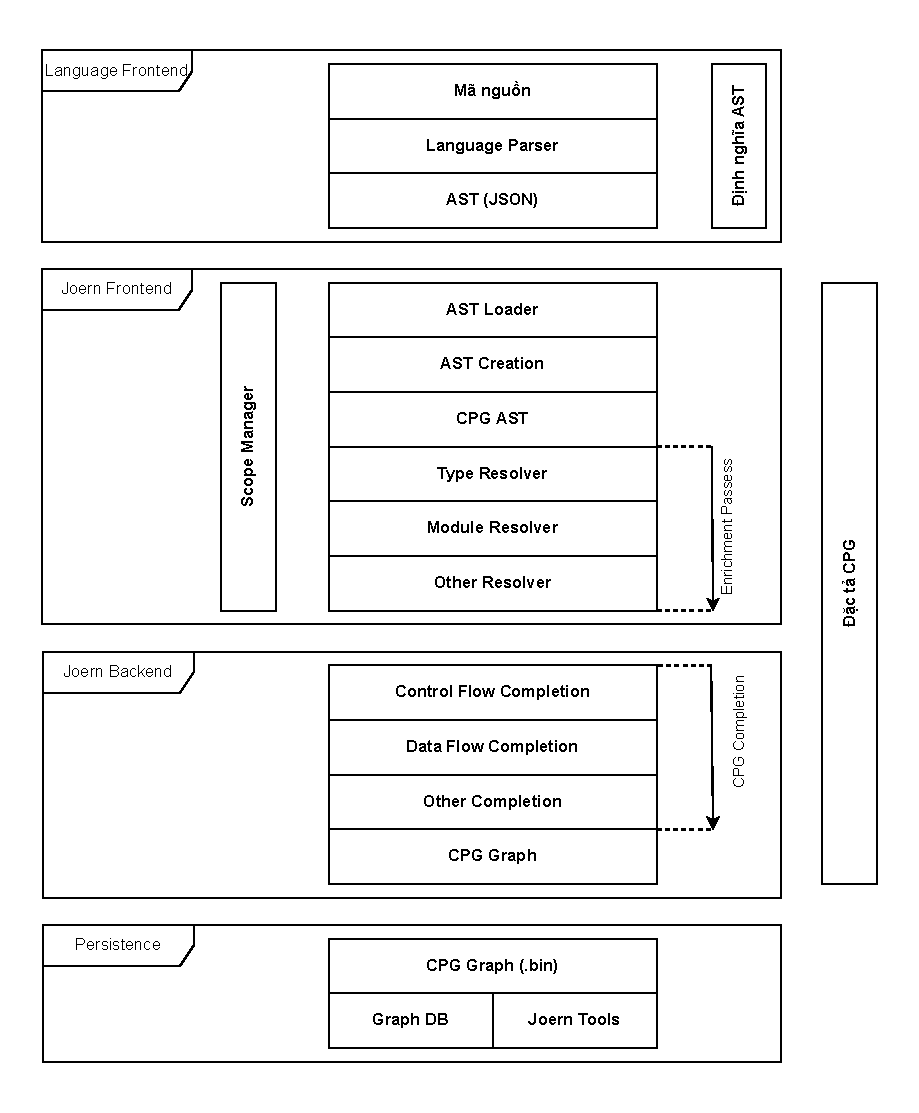
\includegraphics[width=1\columnwidth]{figures/c3/c3_arch.drawio.pdf}
	\centering
	\caption{Kiến trúc công cụ.}
	\label{img:c3_arch}
\end{figure}

Do sử dụng công cụ joern nên kiến trúc của công cơ về cơ bản sẽ là kiến trúc của Joern và mở rộng thêm. Phần này sẽ đi chi tiết hơn so với phần \ref{sec:joern_flow} đã trình bày ở phía trên. Các thành phần chính của công cụ bao gồm:

\textbf{Language Frontend} là phần đặc thù của mỗi ngôn ngữ lập trình, người dùng cần tự đảm nhiệm phần này khi muốn mở rộng công cụ Joern cho ngôn ngữ lập trình mới. Nhiệm vụ của Language Frontend là chuyển đổi mã nguồn thành cây AST dựa trên định nghĩa AST của đặc tả ngôn ngữ. Language Frontend có thể được cài đặt bằng bất cứ ngôn ngữ nào, do đó để có thể chuyển tiếp dư liệu cho quá trình tiếp theo, Language Frontend cần xuất cây AST ra dữ liệu trung gian, ở đây là JSON.

\textbf{Joern Frontend} là nơi chính thực hiện các công việc chuyển đổi cây AST của một ngôn ngữ lập trình cụ thể thành cây CPG theo đặc tả CPG. Đặc tả CPG sẽ được sử dụng xuyên suốt trong cả Joern Frontend và Joern Backend.
Joern Frontend sẽ nhận dữ liệu từ Language Frontend dưới dạng JSON bằng AST Loader. Cây AST sau khi được nạp vào Joern Frontend dưới ngôn ngữ Scala thì sẽ được chuyển đổi thành cây CPG bởi AST Creation. AST Creation thực hiện ánh xạ mỗi một loại nút AST của ngôn ng
sang một loại nút CPG tương ứng. Không chỉ tạo nút, AST Creation còn tạo các cạnh giữa các nút, giữa các nút có thể có nhiều cạnh, mỗi cạnh thể hiện một mối quan hệ giữa các nút. Mặc định giữa các nút có mối quan hệ là cạnh \textit{AST}. Tùy vào thể loại nút thì sẽ có các cạnh thể hiện mối quan hệ khác, ví dụ nút IF sẽ có cạnh \textit{CONDITION} nối với nút thể hiện điều kiện của IF.

\textbf{Scope Manager} được sử dụng trong Joern Frontend để thực hiện quản lý phạm vi của các biến, hàm hay các khai báo khác. Trong phần lớn các ngôn ngữ, một đơn vị cấu trúc sẽ có định danh riêng và định danh đó chỉ hợp lệ trong 1 giới hạn nhất định. Trong quá trình duyệt cây AST, Scope Manager sẽ kiểm soát thông tin về các định danh và phạm vi hoạt động của chúng. Khi sử dụng một định danh hoặc khai báo một định danh mới, Scope Manager sẽ kiểm tra xem khai báo đó có hợp lệ trong phạm vi hay không. Với Scope Manager ta có thể xác định được quan hệ giữa việc khai báo và sử dụng một biến, hàm hay đơn vị cấu trúc khác, từ đó có thể xác định được các cạnh giữa các nút trong cây CPG. Các cạnh sau này sẽ được sử dụng để xây dựng đồ thị CFG và PDG.

\textbf{Pass.} Như đã đề cập ở trên, một phần của cây AST CPG bao gồm các nút và cạnh đã được xây dựng ở AST Creation kết hợp với Scope Manager. Sau đó cây AST CPG sẽ tiếp tục được làm giàu thông tin bằng cách đi qua các Pass. Mỗi Pass sẽ bổ sung một lớp thông tin riêng biệt, ví dụ thông tin về kiểu dữ liệu, cấu trúc module, thứ tự thực hiện câu lệnh, ... Các lớp thông tin này hoàn toàn phụ thuộc vào ngữ cảnh của ngôn ngữ, do vậy số lượng pass cũng sẽ không cố định. Các pass thao tác trên AST CPG nên có thể dùng chung cho nhiều ngôn ngữ, nhưng cũng có các pass được xây dựng riêng cho đặc điểm của một ngôn ngữ cụ thể. Một pass có thể phụ thuộc vào kết quả của pass trước đó hoặc chạy độc lập nên thứ tự chạy các pass cũng rất quan trọng. Ở đây, công cụ chỉ sử dụng 2 pass là Type Resolver và Module Resolver để xử lý kiểu dữ liệu và hệ thống module của Rust, các pass khác sẽ được xây dựng trong tương lai. Sau khi chạy qua các pass, cây AST CPG đã được bổ sung các lớp thông tin nhất định và đây cũng là công đoạn cuối cùng của Joern Frontend.

\textbf{Joern Backend}. Khi chuyển đổi một ngôn ngữ sang CPG, người dùng phải tự thực hiện công đoạn Language Frontend và Joern Frontend để xây dựng cây CPG. Các thông tin có được từ 2 bước trên sẽ được Joern Backend sử dụng để tự động hoàn thiện cây AST CPG thành đồ thị CPG. Các nút, cạnh mới về luồng điều khiển, luồng dữ liệu sẽ được thêm vào và kết nối với các cạnh, nút đã tồn tại. Không chỉ lớp thông tin về điều khiển và dữ liệu, Joern Backend bổ sung các lớp thông tin như  FileSystem, CallGraph, Shortcuts, TagsAndLocation, Annotation \cite{joernCodeProperty}. Kết quả cuối cùng của Joern Backend là một đồ thị CPG hoàn chỉnh.

\textbf{Persistence}. Đồ thị CPG có thể được lưu trư bền vững dưới dạng file nhị phân. File này có thể tiếp tục được chuyển đổi thành kiểu dữ liệu tương thích với các công cụ khác như Neo4j để thực hiện các truy vấn phức tạp hơn, hoặc sử dụng bằng các công cụ khác của Joern.

\section{Chuyển đổi các cú pháp Rust sang đồ thị CPG}

Phần này sẽ trình bày một số cú pháp của Rust khác biệt so với ngôn ngữ C/C++ và cách mà công cụ đã chuyển đổi sang đồ thị CPG cho các cú pháp này.
Các cú pháp bao gồm: if let, while let, match, lifetime.
Những đoạn mã nguồn và hình ảnh mô tả đồ thị CPG được sử dụng từ giờ đến cuối khóa luận sẽ được đơn giản hóa để dễ dàng thể hiện và minh họa.
Các cạnh và các nút không phải trọng tâm của đồ thị CPG sẽ được loại bỏ để tập trung vào các tính năng cần trình bày.

\subsection{Cú pháp if let}
If else là cấu trúc điều khiển có mặt trong tất cả các loại ngôn ngữ phổ biến.
% Nó cho phép chúng ta kiểm tra một điều kiện và thực thi một khối mã nếu điều kiện đúng và một khối mã khác nếu điều kiện sai.
Cấu trúc câu lệnh if else sẽ bao gồm một điều kiện và 2 khối mã.
Nếu điều kiện đúng, khối mã trong if sẽ được thực thi, ngược lại khối mã trong else sẽ được thực thi.
Thông thường khối điều kiện sẽ là biểu thức trả về kết quả đúng hoặc sai của biểu thức đó.
Trong ngôn ngữ như C/C++ thì chỉ chấp nhận biểu thức điều kiện, việc sử dụng mệnh đề (có dấu hai chấm để kết thúc câu lệnh) là không hợp lệ.
Với phương châm "Expression over statement" và nhằm mục đích tạo sự ngắn gọn, Rust cho phép thực hiện phép khai báo biến và gán giá trị cho biến trong cùng một câu lệnh bằng điều kiện if let.
Cú pháp tổng quát của câu lệnh if let như sau:

\begin{listing}[H]
\begin{minted}[mathescape, breaklines, frame=lines, framesep=2mm, baselinestretch=1.2, fontsize=\footnotesize, linenos]{rust}
if let <pattern> = <expression> {
     <block>
} else {
     <block>
}
\end{minted}
\caption{Mã giả cho cú pháp tổng quát của if let.}
\label{code:c4_iflet_general}
\end{listing}

Cú pháp \ref{code:c4_iflet_general} sẽ thực hiện 2 công việc.
Thứ nhất là kiểm tra xem \texttt{<expression>} có khớp với \texttt{<pattern>} hay không, nếu không khớp thì trả về $false$, nếu khớp thì trả về $true$.
Thứ hai là khai báo các biến mới từ \texttt{<pattern>} nếu điều kiện thành công, các biến sẽ có phạm vi tồn tại trong khối lệnh điều kiện thành công.
% thì tiếp tục thực hiện tạo biến mới dựa theo \texttt{<pattern>}

\begin{listing}[H]
\begin{minted}[mathescape, breaklines, frame=lines, framesep=2mm, baselinestretch=1.2, fontsize=\footnotesize, linenos]{rust}
let number: Option<i32> = None;

if let Some(i) = number {
    println!("Matched number {:?}!", i);
} else {
    // ...
}
\end{minted}
\caption{Ví dụ mã nguồn cho cú pháp if let.}
\label{code:c4_iflet}
\end{listing}

Đoạn mã \ref{code:c4_iflet} sử dụng cú pháp if let với điều kiện là kiểm tra xem biến \texttt{number} có giá trị bên trong hay không, nếu có thì khai báo một biến \texttt{i} mới và gán giá trị cho biến \texttt{i}.
Tiếp theo sẽ thực thi khối lệnh bên trong if.
Biến \texttt{i} sẽ chỉ tồn tại trong khối lệnh if, và được sử dụng trong câu lệnh \texttt{println!}.
Do thực hiện 2 công việc trong cùng 1 câu lệnh nên khi quy đổi sang câu lệnh tương tự trong ngôn ngữ C/C++, cú pháp if let sẽ tương đương 2 câu lệnh kiểm tra điều kiện và gán biến \ref{code:c4_iflet_cpp}.

\begin{listing}[H]
\begin{minted}[mathescape, breaklines, frame=lines, framesep=2mm, baselinestretch=1.2, fontsize=\footnotesize, linenos]{cpp}
Object* obj = inputObj();

if (obj != nullptr) { // 1 câu lệnh kiểm tra điều kiện
    int number = *static_cast<int*>(obj); // 1 câu lệnh gán biến
    std::cout << "Matched " << number << "!" << std::endl;
}
\end{minted}
\caption{Ví dụ mã nguồn cho cú pháp if let tương đương trong C++.}
\label{code:c4_iflet_cpp}
\end{listing}

\begin{figure}[H]
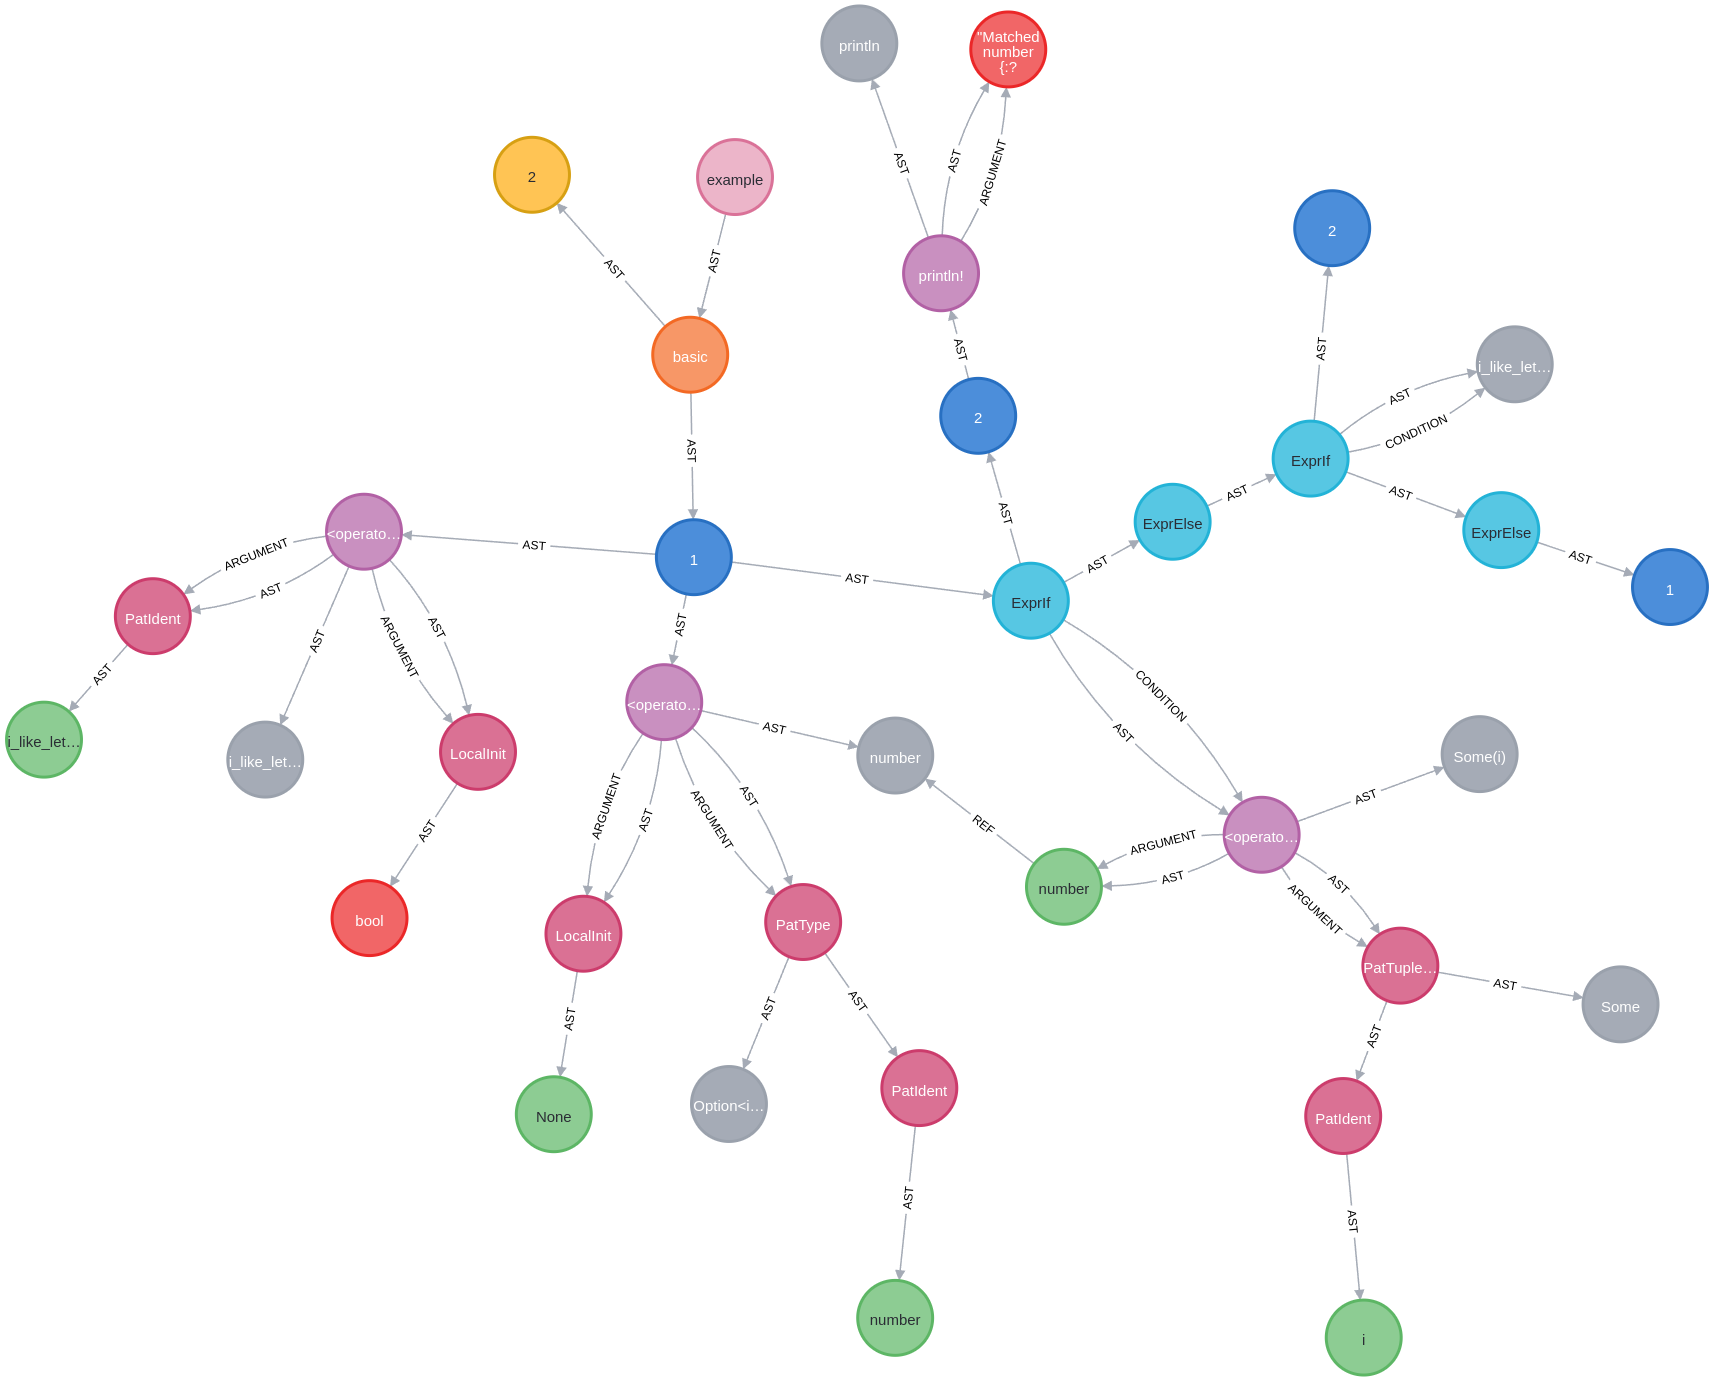
\includegraphics[width=1\columnwidth]{figures/c4/c4_iflet.png}
\centering
\caption{Ví dụ đồ thị CPG cho đoạn mã nguồn của cú pháp if let \ref{code:c4_iflet}.}
\label{img:c4_cpg_iflet}
\end{figure}

% Trong Hình \ref{img:c4_cpg_iflet}, cạnh \texttt{CONDITION} của nút \texttt{ExprIf} trỏ tới nút \texttt{Assignment}, đồng thời cũng khai báo biến mới với tên \texttt{i}. Mặc định, Joern sẽ không cho phép cạnh \texttt{CONDITION} trỏ tới nút \texttt{Assignment} bởi vì trong ngôn ngữ C/C++ không thể lấy một phép gán làm điều kiện. Tuy nhiên, khóa luận đã thực hiện chỉnh sửa đặc tả CPG của Joern để cho phép cạnh \texttt{CONDITION} trỏ tới nút \texttt{Assignment} trong trường hợp này.
% Điều chỉnh này giúp mô hình hóa chính xác hơn ngữ nghĩa của các ngôn ngữ hỗ trợ khai báo biến trực tiếp trong khối điều kiện, như Rust. Các mệnh đề trong khối điều kiện đúng được thực thi, nếu có sử dụng tới biến \texttt{i} thì sẽ tham chiếu tới biến \texttt{i} vừa được khai báo thông qua cạnh \texttt{REF}. Nhờ đó, đồ thị CPG không chỉ phản ánh chính xác cấu trúc mã nguồn mà còn đảm bảo khả năng truy vấn và phân tích đúng các phụ thuộc dữ liệu trong các ngữ cảnh tương tự.

Trong Hình \ref{img:c4_cpg_iflet}, cạnh \texttt{CONDITION} của nút \texttt{ExprIf} trỏ tới nút \texttt{Assignment}, đồng thời cũng khai báo biến mới với tên \texttt{i}.
Mặc định, Joern sẽ không cho phép cạnh \texttt{CONDITION} trỏ tới nút \texttt{Assignment} bởi vì trong ngôn ngữ C/C++ không thể lấy một phép gán làm điều kiện.
Tuy nhiên, khóa luận đã thực hiện chỉnh sửa đặc tả CPG của Joern để cho phép cạnh \texttt{CONDITION} trỏ tới nút \texttt{Assignment} trong trường hợp này.
Điều chỉnh này giúp mô hình hóa chính xác hơn ngữ nghĩa của các ngôn ngữ hỗ trợ khai báo biến trực tiếp trong khối điều kiện như Rust.
Các mệnh đề trong khối điều kiện đúng được thực thi, nếu có sử dụng tới biến \texttt{i} thì sẽ tham chiếu tới biến \texttt{i} vừa được khai báo thông qua cạnh \texttt{REF}.

\subsection{Cú pháp while let}

% Tương tự với tính năng if let ở trên, Rust cũng hỗ trợ việc khai báo biến làm điều kiện cho vòng lặp while.
% Cú pháp của vòng lặp while let như sau:

% \begin{minted}[mathescape, breaklines, frame=lines, framesep=2mm, baselinestretch=1.2, fontsize=\footnotesize, linenos]{rust}
% while let <pattern> = <expression> {
%         <block>
% }
% \end{minted}


\begin{listing}[H]
\begin{minted}[mathescape, breaklines, frame=lines, framesep=2mm, baselinestretch=1.2, fontsize=\footnotesize, linenos]{rust}
let mut optional = Some(0);

while let Some(i) = optional {
    if i > 9 {
        optional = None;
    } else {
        optional = Some(i + 1);
    }
}
\end{minted}
\caption{Ví dụ mã nguồn cho cú pháp while let.}
\label{code:c4_whilelet}
\end{listing}

Tương tự với cú pháp if let ở trên, Rust cũng hỗ trợ việc khai báo biến làm điều kiện cho vòng lặp while.
Đoạn mã \ref{code:c4_whilelet} trên được hiểu là nếu biến \texttt{optional} có giá trị bên trong thì thực hiện vòng lặp, nếu không thì kết thúc vòng lặp.
Đồng thời, sẽ có một biến \texttt{i} mới được khởi tạo đối với mỗi lần lặp, giá trị của \texttt{i} bằng giá trị của số nguyên bên trong biến \texttt{optional}.
Các mệnh đề trong khối được thực thi, và nếu có sử dụng tới, chúng sẽ tham chiếu tới biến \texttt{i} vừa được khai báo thông qua cạnh \texttt{REF}.
Không chỉ vậy, vế phải của điều kiện có thể được gán lại liên tục trong quá trình lặp, đảm bảo vòng lặp kiểm tra trạng thái mới của biến \texttt{optional} sau mỗi lần lặp.
Nhờ vậy thể hiện được các thay đổi động của dữ liệu trong suốt quá trình thực thi vòng lặp.
Khi việc kiểm tra giá trị số nguyên bên trong biến \texttt{optional} thất bại, vòng lặp sẽ kết thúc.
% , đảm bảo hành vi nhất quán với ngữ nghĩa của mã nguồn Rust.

Hình \ref{img:c4_cpg_whilelet} mô tả đồ thị CPG cho đoạn mã nguồn while let ở trên.
Nút \texttt{CONTROL STRUCTURE} thể hiện vòng lặp while, trong khi nút \texttt{ASSIGNMENT} biểu diễn điều kiện của vòng lặp và được nối với nút \texttt{CONTROL STRUCTURE} thông qua cạnh \texttt{CONDITION}
Ngoài ra, biến \texttt{i} được khai báo riêng tại nút \texttt{LOCAL} và tham chiếu thông qua cạnh \texttt{REF} bởi các nút tương ứng với các mệnh đề trong khối mã.

\begin{figure}[H]
    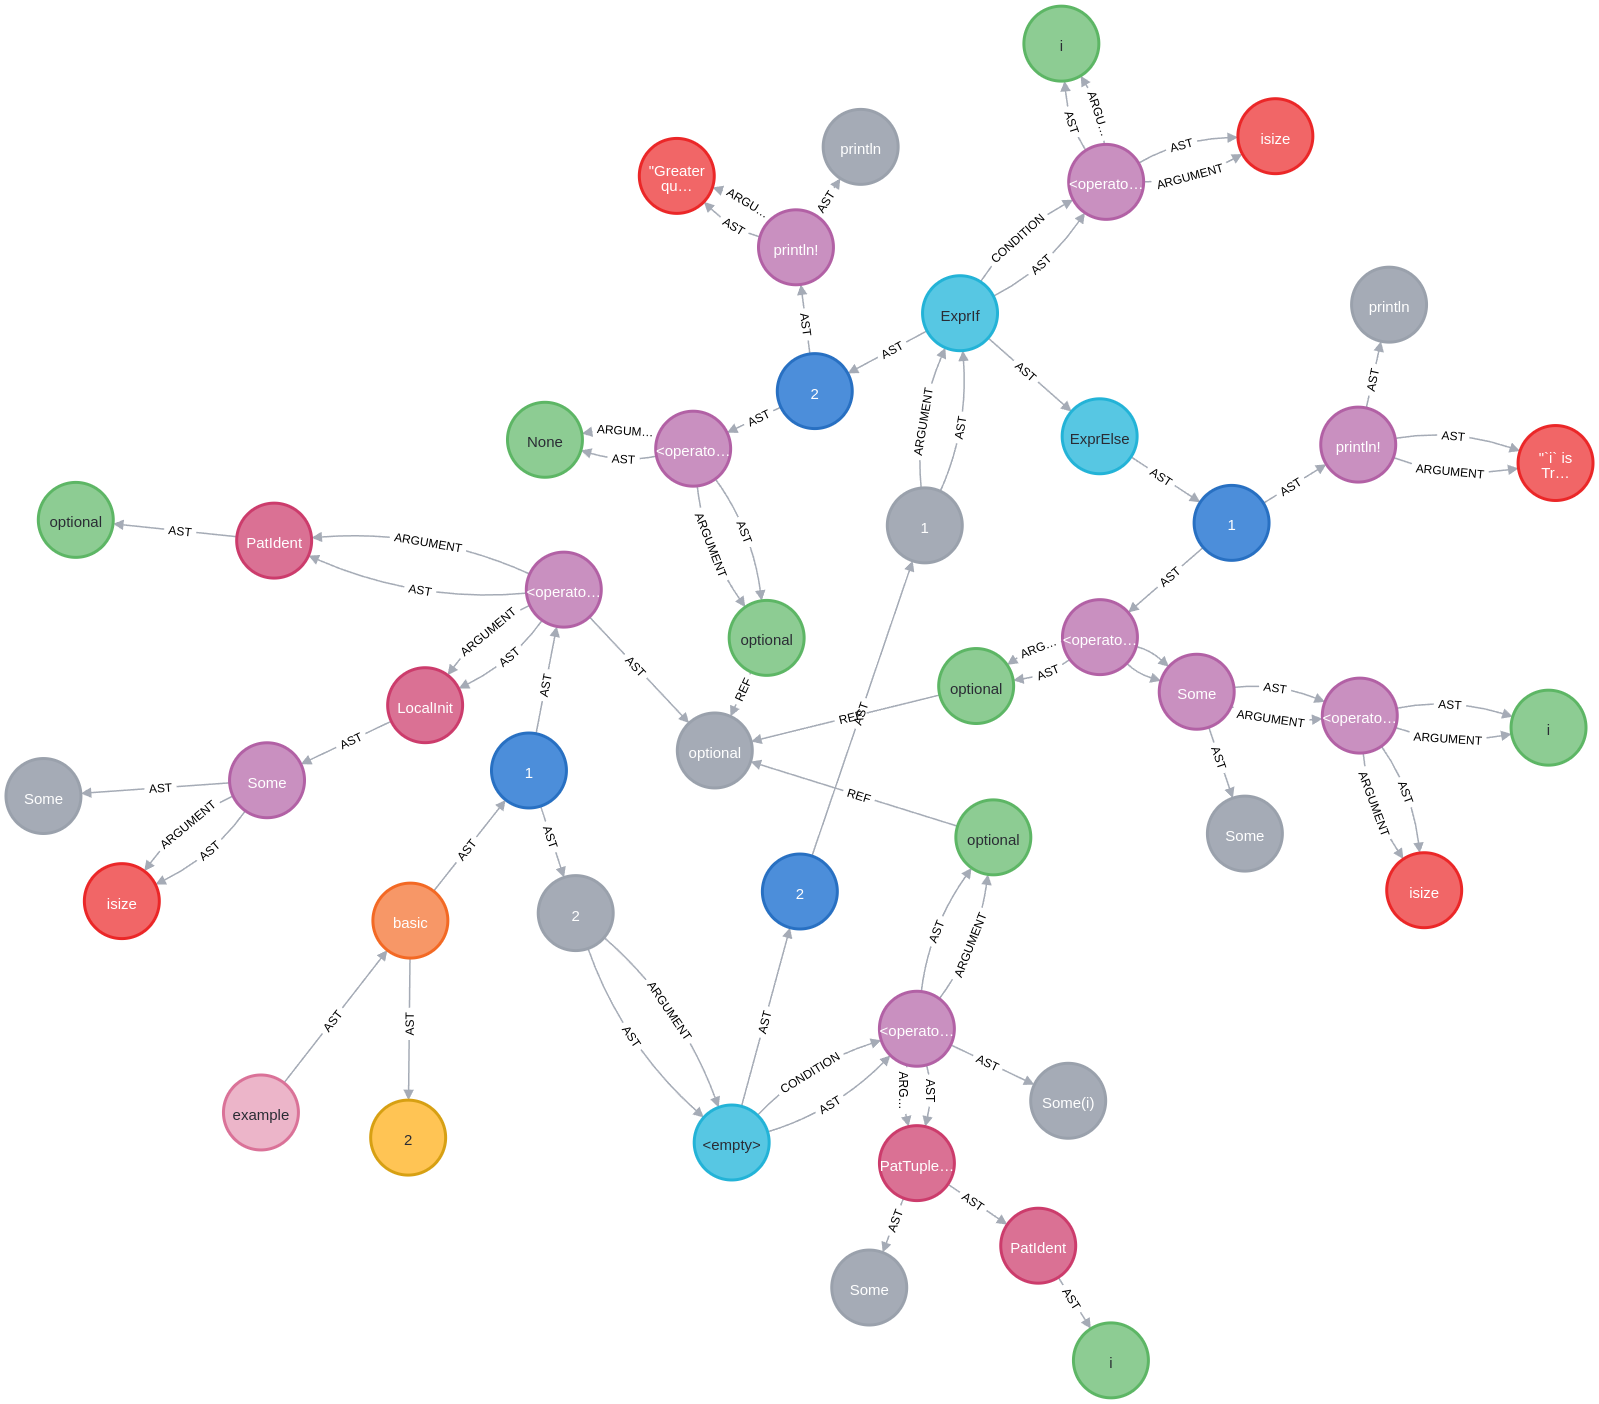
\includegraphics[width=1\columnwidth]{figures/c4/c4_whilelet.png}
    \centering
    \caption{Ví dụ đồ thị CPG cho đoạn mã nguồn cú pháp while let \ref{code:c4_whilelet}.}
    \label{img:c4_cpg_whilelet}
\end{figure}

\subsection{Cú pháp match}

Ngoài việc sử dụng mệnh đề gán biến thành biểu thức điều kiện, tính hướng hàm của Rust còn thể hiện ở sự kết hợp giữa cơ chế pattern matching và kiểu dữ liệu đại số.
Ví dụ \ref{code:c4_match} cho thấy cấu trúc match không chỉ kiểm tra giá trị mà còn kết hợp với các mẫu phức tạp, bao gồm kiểm tra điều kiện, kiểm tra các kiểu dữ liệu khác nhau và so sánh.
Điều này mang lại cho Rust tính linh hoạt cao hơn so với switch trong C/C++ khi chỉ so sánh giá trị nguyên thủy.
Một điểm khác biệt quan trọng giữa match và switch là tính toàn diện của match.
Rust yêu cầu các mẫu trong match phải bao quát tất cả các khả năng có thể xảy ra, nếu không trình biên dịch sẽ báo lỗi.
Điều này giúp đảm bảo rằng không có tình huống nào bị bỏ qua, tăng cường độ an toàn của mã nguồn.
Trong khi đó, switch trong C/C++ không yêu cầu bao quát tất cả các trường hợp, và việc bỏ sót một trường hợp có thể dẫn đến lỗi hoặc hành vi không mong muốn.
Thêm vào đó, match trong Rust cho phép trích xuất và xử lý các thành phần của cấu trúc dữ liệu phức tạp ngay trong quá trình đối chiếu mẫu.
% Ví dụ, Rust có thể match trên \texttt{tuple}, \texttt{enum}, \texttt{struct}, trong khi switch của C/C++ thường chỉ giới hạn trong các giá trị nguyên thủy.
Cú pháp match có thể thực hiện trên \texttt{tuple}, \texttt{enum}, \texttt{struct}, trong khi switch của C/C++ chỉ giới hạn cho các giá trị nguyên thủy.

\begin{listing}[H]
\begin{minted}[mathescape, breaklines, frame=lines, framesep=2mm, baselinestretch=1.2, fontsize=\footnotesize, linenos]{rust}
enum Color {
    Red,
    Blue(u32, u32, u32),
    Green {
        red: u32,
        green: u32,
        blue: u32,
    },
}

fn main() {
    let color = Color::Blue(0, 0, 255);

    match color {
        Color::Red =>
            println!("The color is Red!")
        Color::Blue(r, g, b) =>
            println!("R: {}, G: {}, B: {}!", r, g, b)
        Color::Green {red, green, blue} =>
            println!("R: {}, G: {}, B: {}!", red, green, blue),
    }
}
\end{minted}
\caption{Ví dụ mã nguồn cho cú pháp match.}
\label{code:c4_match}
\end{listing}

Trong Hình \ref{img:c4_match}, các biến thể của \texttt{enum Color} được thể hiện bằng nút \texttt{VARIANT}.
Biến thể \texttt{Red} do không có giá trị nên không có nút con nào khác.
Biến thể \texttt{Blue} có giá trị là 3 số nguyên tính theo chỉ mục nên sẽ có 3 nút con \texttt{MEMBER} tương ứng, nhưng mỗi nút \texttt{MEMBER} này không có nút con \texttt{IDENTIFIER} chỉ ra tên thành phần.
Ngược lại mỗi nút \texttt{MEMBER} của \texttt{Green} sẽ có nút con \texttt{IDENTIFIER} thể hiện tên của thành phần.
Còn cú pháp match được thể hiện bằng nút \texttt{CONTROL STRUCTURE} và cạnh \texttt{CONDITION} nối với nút \texttt{IDENTITER} chi tới biến \texttt{color}.
Mỗi trường hợp của match sẽ được thể hiện bằng nút \texttt{ARM} và mỗi \texttt{ARM} cũng có sẽ cạnh \texttt{CONDITION} nối tới nút thể hiện biểu thức điều kiện.

\begin{figure}[H]
    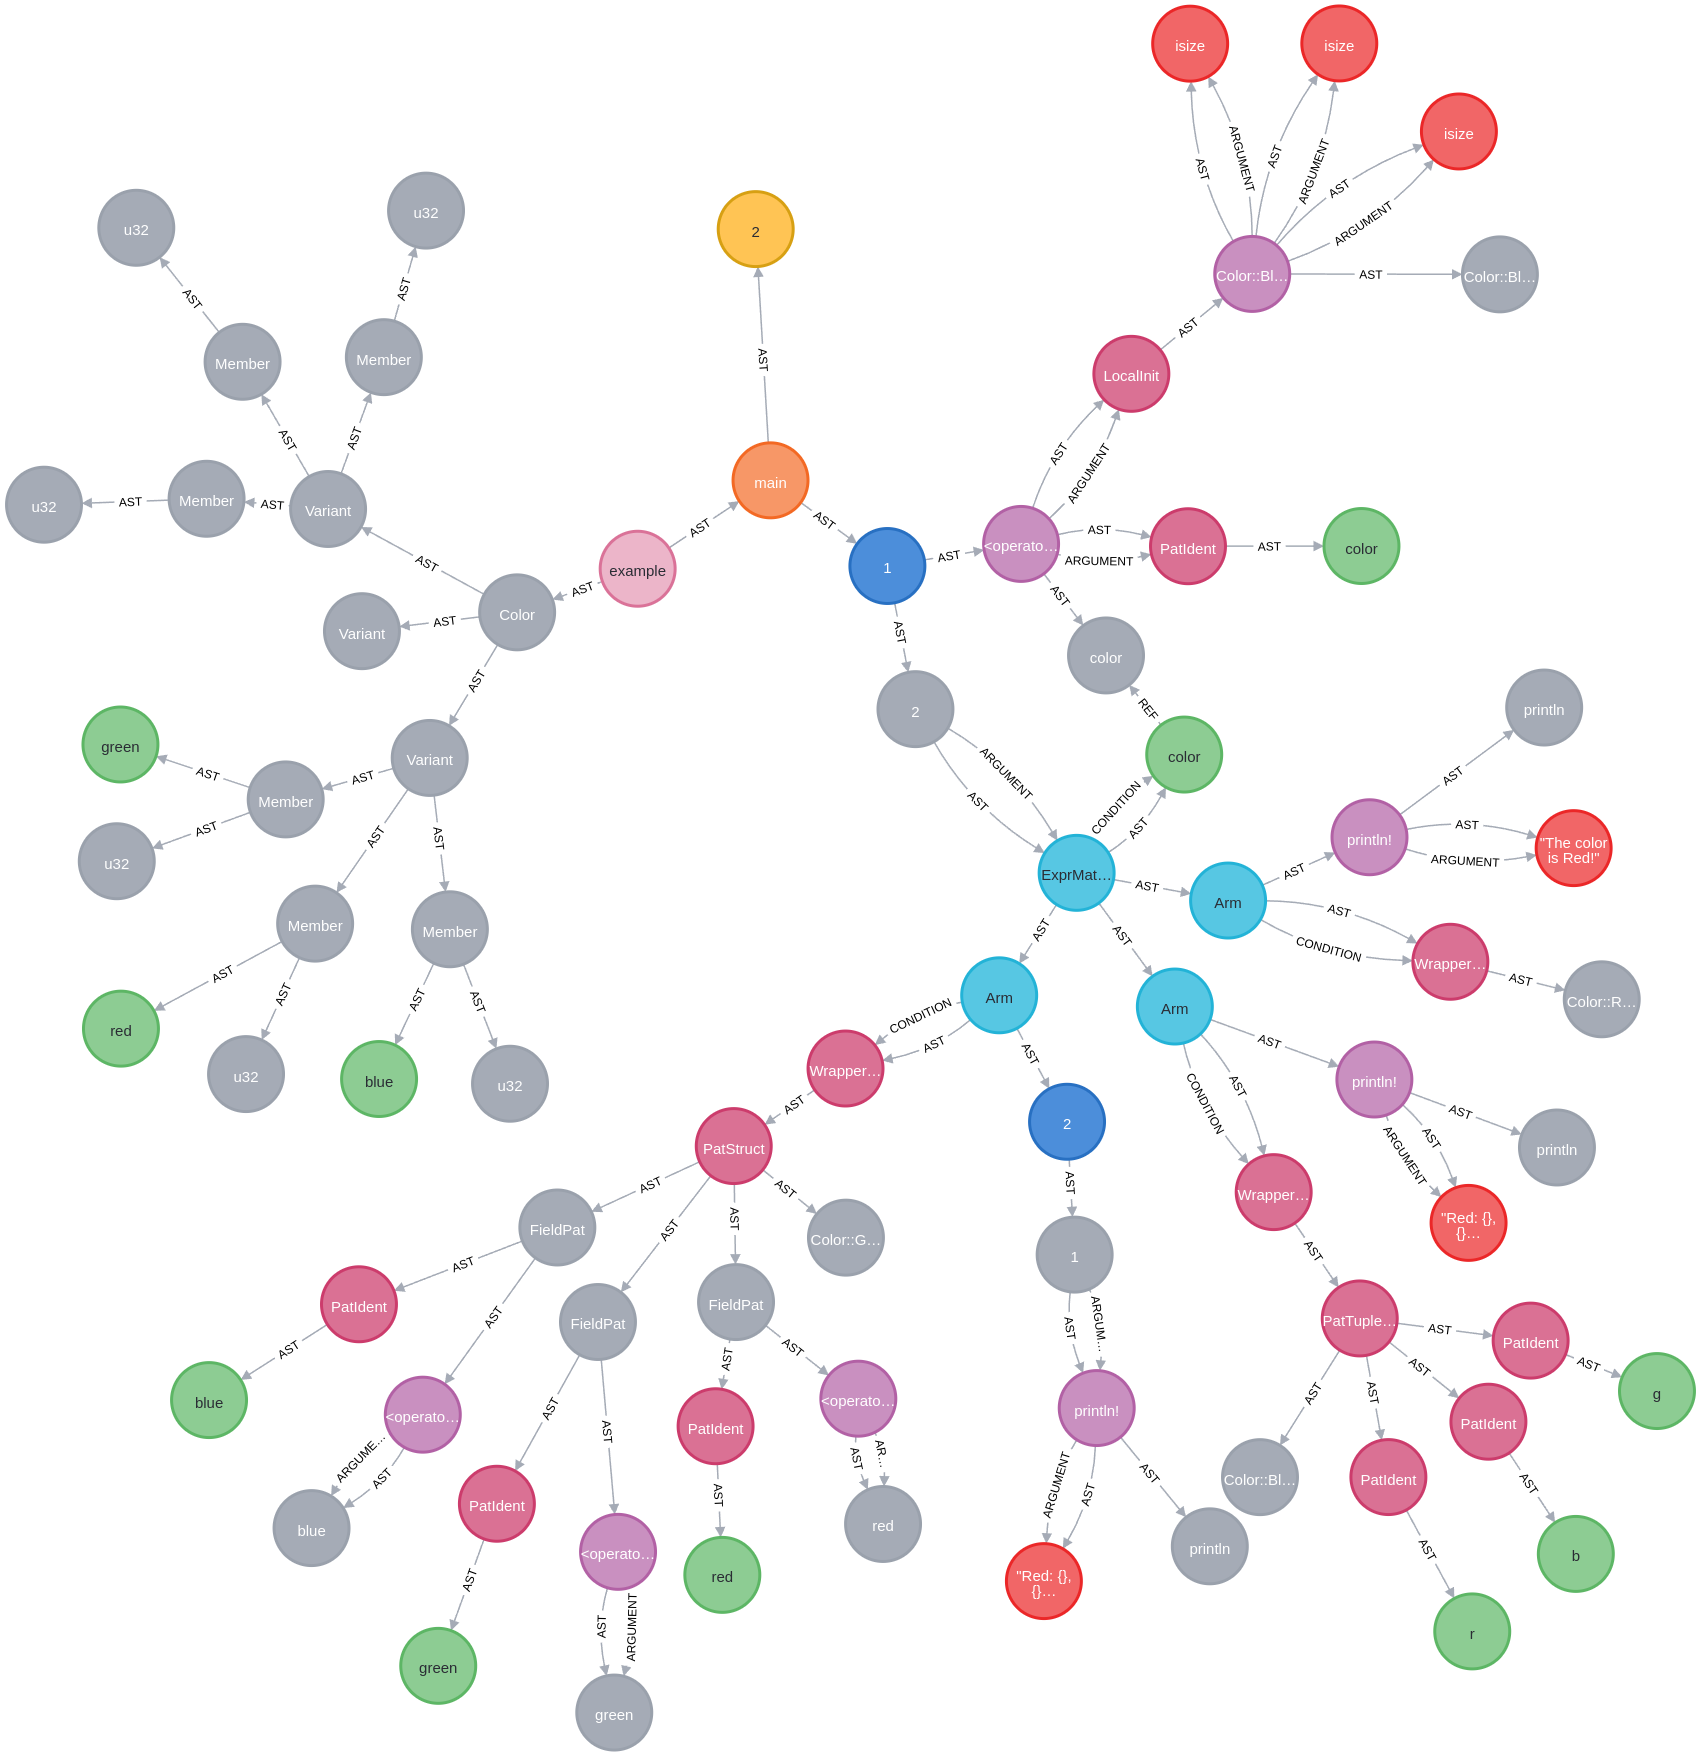
\includegraphics[width=1\columnwidth]{figures/c4/c4_match.png}
    \centering
    \caption{Ví dụ đồ thị CPG cho đoạn mã nguồn cú pháp match \ref{code:c4_match}.}
    \label{img:c4_match}
\end{figure}

\subsection{Cú pháp lifetime}

Lifetime là cơ chế được sử dụng trong Rust để quản lý vòng đời của các biến tham chiếu.
Quản lý lifetime một cách chặt chẽ đảm bảo rằng các biến tham chiếu không trỏ tới vùng nhớ không còn tồn tại.
Lifetime có vai trò tương tự như kiểu tổng quát, nhưng thay vì định kiểu cho biến thì lifetime sẽ xác định thời gian hợp lệ cho biến tham chiếu.
Để biểu diễn được kiểu dữ liệu tổng quát, đặc tả CPG của Joern đã có các nút như \texttt{TYPE}, \texttt{TYPE PARAMETER}, \texttt{TYPE ARGUMENT}.
Do vậy để biểu diễn được tính năng lifetime trên đồ thị CPG, 3 loại nút mới đã được thêm vào đặc tả CPG bao gồm \texttt{LIFETIME}, \texttt{LIFETIME PARAMETER}, \texttt{LIFETIME ARGUMENT}.
Để chỉ ra quan hệ ràng buộc giữa biến và lifetime hay quan hệ giữa các lifetime với nhau, ta sẽ thêm cạnh \texttt{OUT LIVE}.
Cạnh \texttt{OUT LIVE} mang ý nghĩa nút nguồn phải có thời gian hợp lệ lớn hơn nút đích. Quy định về thời gian hợp lệ của một đơn vị thành phần so với đơn vị thành phần khác được tham khảo từ Rust Reference.

Nút \texttt{LIFETIME PARAMETER} và \texttt{LIFETIME ARGUMENT} được sử dụng cho các \texttt{struct}, \texttt{enum}, \texttt{trait} để chỉ ra lifetime tổng quát cho các biến tham chiếu.
Loại nút \texttt{LIFETIME} sẽ thể hiện vòng đời thực sự của biến tham chiếu.
Các biến tham chiếu sẽ được gán lifetime thông qua việc sử dụng dấu "\texttt{'}" đi trước tên lifetime, ví dụ như \texttt{'a}.
Nếu biến đánh dấu lifetime \texttt{'a} thì sẽ có cạnh \texttt{OUT LIVE} trỏ từ nút \texttt{IDENTIFIER} của biến tới nút \texttt{LIFETIME} đại diện cho \texttt{'a} tương ứng.
Nếu lifetime \texttt{'a} được giới hạn bởi lifetime \texttt{'b} thì sẽ có cạnh \texttt{OUT LIVE} từ nút \texttt{LIFETIME} \texttt{'a} tới nút \texttt{LIFETIME} \texttt{'b}.

% Lifetime elision là cơ chế trong Rust giúp tự động suy diễn lifetime cho các biến tham chiếu.
% Có ba luật chính về lifetime elision trong Rust.
% Thứ nhất, mỗi biến tham chiếu đầu vào sẽ được tự động gán lifetime mà không cần phải đánh dấu một cách tường minh.
% Thứ hai, nếu hàm có chỉ có một biến tham chiếu đầu và một biến tham chiếu đầu ra, trình biên dịch sẽ suy luận rằng biến tham chiếu đầu ra có cùng lifetime với biến tham chiếu đầu vào.
% Cuối cùng, nếu hàm có một hoặc nhiều hơn một biến tham chiếu đầu vào và một trong biến đầu vào là biến \texttt{self} (\texttt{self} tương đương với \texttt{this} trong C/C++), trình biên dịch sẽ suy luận rằng biến tham chiếu đầu ra có cùng lifetime với \texttt{self}.
% Ngoài 3 trường hợp trên, Rust yêu cầu phải ghi rõ lifetime cho tất cả các biến tham chiếu để tránh nhầm lẫn và đảm bảo an toàn bộ nhớ.

\begin{listing}[H]
\begin{minted}[mathescape, breaklines, frame=lines, framesep=2mm, baselinestretch=1.2, fontsize=\footnotesize, linenos]{rust}
fn longest<'a>(x: &'a str, y: &'a str) -> &'a str {
    if x.len() > y.len() {
        x
    } else {
        y
    }
}
\end{minted}
\caption{Ví dụ mã nguồn cho lifetime.}
\label{code:c4_lifetime_1}
\end{listing}

Các biến tham chiếu luôn có một lifetime tương ứng với nó, có thể được chỉ ra tường minh hoặc không tường minh.
Đoạn mã \ref{code:c4_lifetime_1} mô tả một ví dụ bắt buộc phải khai báo lifetime một cách tường minh để chỉ rõ vòng đời của biến tham chiếu.
Hàm \texttt{longest} nhận vào 2 biến tham chiếu \texttt{x} và \texttt{y} cùng có lifetime \texttt{'a} và giá trị trả về cũng có lifetime \texttt{'a}.
Trình biên dịch Rust có thể tự động suy diễn lifetime không tường minh cho hai biến tham chiếu đầu vào \texttt{x} và \texttt{y}, nhưng không thể suy diễn được lifetime cho giá trị tham chiếu trả về.
Hơn nữa, giá trị trả về của hàm \texttt{longest} là một trong hai giá trị tham chiếu đầu vào.
Do trình biên dịch không thể biết được trong khi thực thi hàm thì giá trị trả về sẽ trỏ tới vùng nhớ của \texttt{x} hay \texttt{y}, do đó cần phải chỉ rõ lifetime cho giá trị trả về.
Biến \texttt{x} và \texttt{y} cùng có lifetime \texttt{'a} tức là \texttt{x} và \texttt{y} sẽ có một khoảng thời gian mà \texttt{x} và \texttt{y} cùng tồn tại và đặt tên khoảng thời gian đó là \texttt{'a}.
Giá trị đầu ra tồn tại trong khoảng thời gian \texttt{'a} này thì luôn đảm bảo không trỏ tới vùng nhớ không còn tồn tại.
Khi sử dụng hàm, nếu đối số đầu vào hay biến nhận giá trị trả về không thỏa mãn ràng buộc lifetime \texttt{'a} thì trình biên dịch Rust sẽ báo lỗi.

\vspace{\baselineskip}

\begin{figure}[H]
    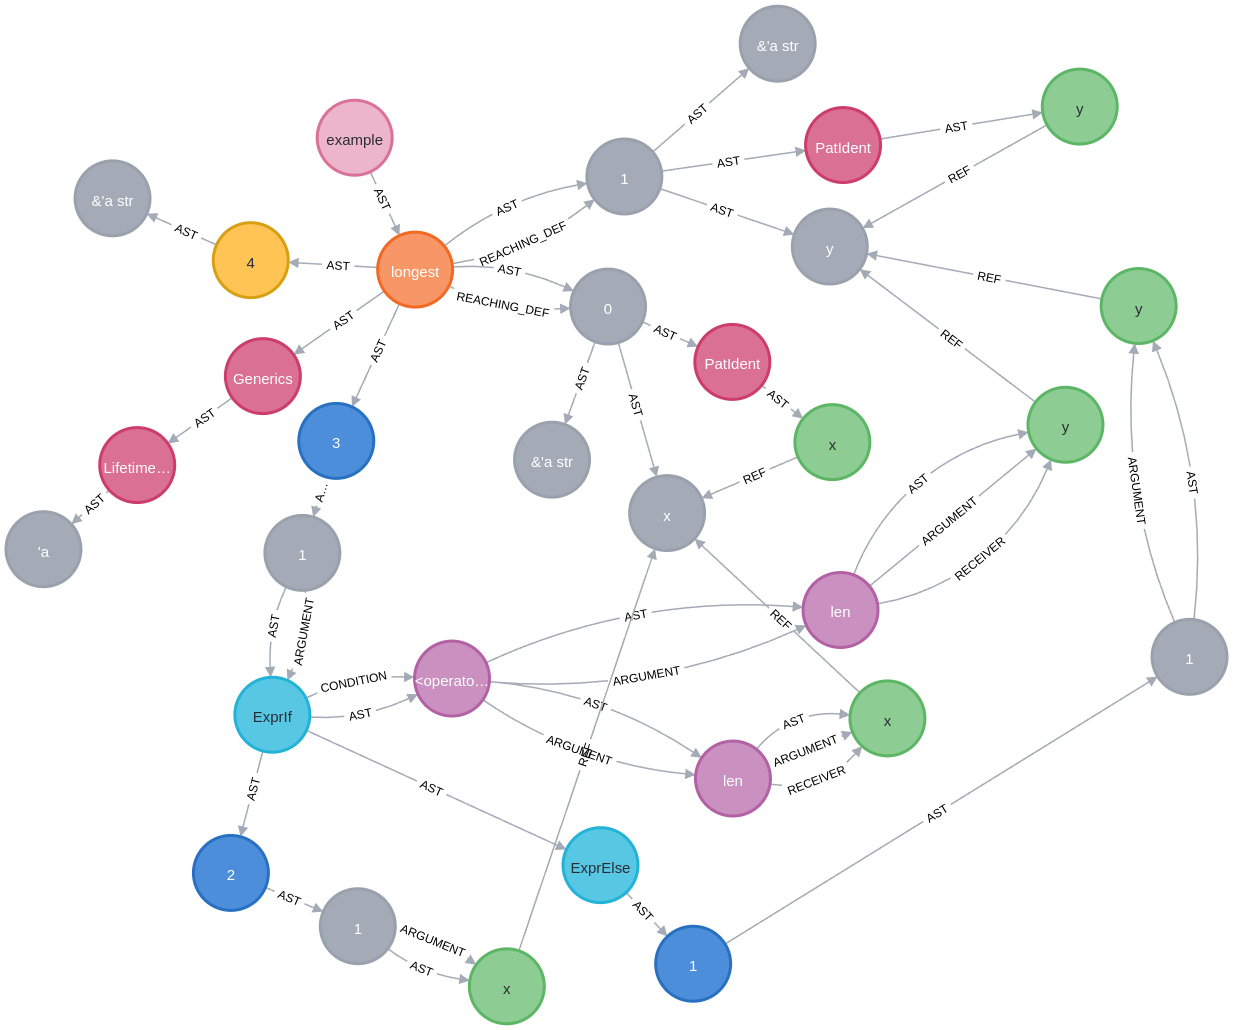
\includegraphics[width=1\columnwidth]{figures/c4/c4_lifetime_1.png}
    \centering
    \caption{Ví dụ đồ thị CPG cho đoạn mã nguồn \ref{code:c4_lifetime_1}.}
    \label{img:c4_lifetime_1}
\end{figure}

Hình \ref{img:c4_lifetime_1} thể hiện mối quan hệ lifetime giữa các biến tham chiếu và giá trị trả về của hàm.
Hàm \texttt{longest} được thể hiện qua nút \texttt{METHOD}.
Trong đó, nút \texttt{METHOD} có cạnh \texttt{AST} trỏ tới nút \texttt{GENERICS}, đại diện cho nút cha bọc lấy nhiều nút thể hiện kiểu tổng quát.
Nút \texttt{LIFETIME PARAMETER} thể hiện lifetime \texttt{'a} của hàm, và cũng là lifetime của các biến tham chiếu và giá trị trả về.
Các biến tham chiếu \texttt{x} và \texttt{y} có cùng lifetime \texttt{'a} được thể hiện qua cạnh \texttt{OUT LIVE} từ nút \texttt{IDENTIFIER} của biến \texttt{x} và \texttt{y} tới nút \texttt{LIFETIME} của \texttt{'a}.
Giá trị trả về của hàm cũng có lifetime \texttt{'a} và được thể hiện qua cạnh \texttt{OUT LIVE} từ nút \texttt{METHOD RETURN} tới nút \texttt{LIFETIME} \texttt{'a}.
Mối quan hệ lifetime giữa các biến tham chiếu và giá trị trả về đều được thể hiện qua các nút \texttt{LIFETIME} và cạnh \texttt{OUT LIVE} trên đồ thị CPG.

\begin{listing}[H]
\begin{minted}[mathescape, breaklines, frame=lines, framesep=2mm, baselinestretch=1.2, fontsize=\footnotesize, linenos]{rust}
fn f<'a, 'b, 'c, T>(x: &'a i32, mut y: &'b i32, z: &'c T)
where
    'b: 'a,
    'c: 'b,
    T: 'b,
{
    // ...
}
\end{minted}
\caption{Ví dụ mã nguồn cho cú pháp lifetime kết hợp cú pháp where.}
\label{code:c4_lifetime_2}
\end{listing}


\begin{figure}[H]
    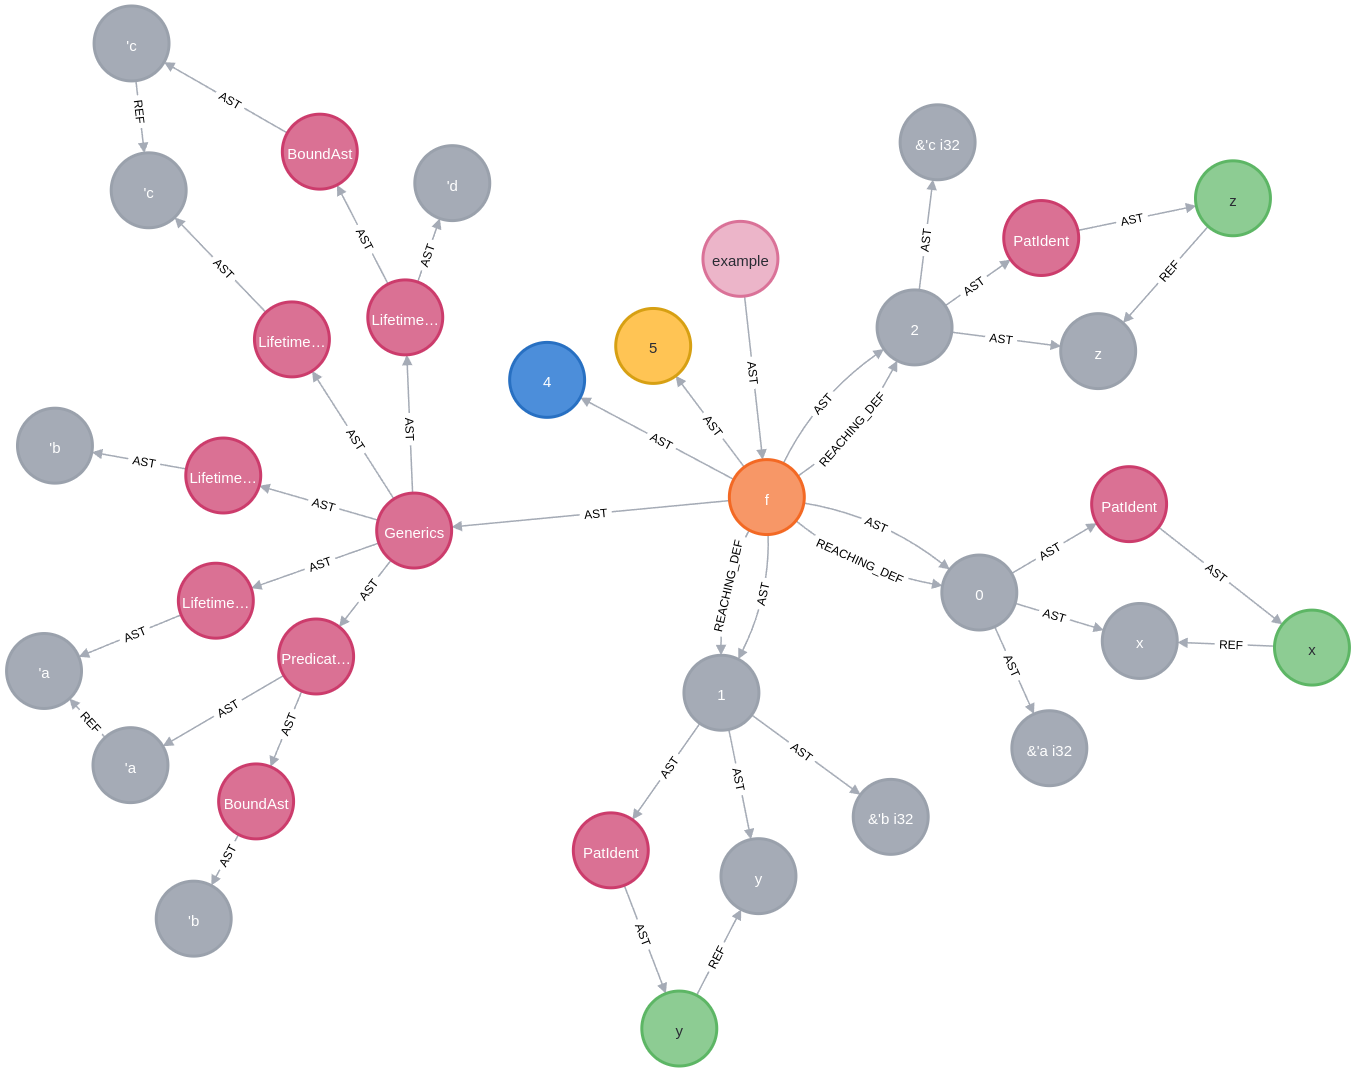
\includegraphics[width=1\columnwidth]{figures/c4/c4_lifetime_2.png}
    \centering
    \caption{Ví dụ đồ thị CPG cho đoạn mã nguồn cú pháp where \ref{code:c4_lifetime_2}.}
    \label{img:c4_lifetime_2}
\end{figure}

Trong Rust, kiểu tổng quát và ràng buộc của nó có thể được chỉ rõ thông qua cú pháp \texttt{where}.
Cú pháp \texttt{where} cho phép thể hiện ràng buộc giữa kiểu dữ liệu tổng quát và kiểu lifetime tổng quát.
Đoạn mã \ref{code:c4_lifetime_2} minh họa về một hàm có nhiều lifetime, nhiều kiểu tổng quát và tham chiếu đầu vào kết hợp với cú pháp \texttt{where} để thể hiện mối quan hệ ràng buộc giữa chúng.
Hàm \texttt{f} nhận vào 3 biến tham chiếu \texttt{x}, \texttt{y}, \texttt{z} có lifetime tương ứng là \texttt{'a}, \texttt{'b}, \texttt{'c}.
Cú pháp \texttt{'b: 'a} thể hiện ràng buộc lifetime \texttt{'b} của biến \texttt{y} phải lớn hơn hoặc bằng lifetime \texttt{'a} của biến \texttt{x}.
Trên đồ thị CPG ở Hình \ref{img:c4_lifetime_2}, điều này tức là sẽ có cạnh \texttt{OUT LIVE} từ nút \texttt{LIFETIME} \texttt{'b} tới nút \texttt{LIFETIME} \texttt{'a}.
Điều này tương tự với việc lifetime \texttt{'c} của biến \texttt{z} phải lớn hơn hoặc bằng lifetime \texttt{'b} của biến \texttt{y}.
Cạnh \texttt{OUT LIVE} từ nút \texttt{LIFETIME} \texttt{'c} tới nút \texttt{LIFETIME} \texttt{'b} được thể hiện rõ ràng trên đồ thị CPG.

Không chỉ ràng buộc giữa các lifetime với nhau, hoàn toàn có thể ràng buộc lifetime cho một kiểu dữ liệu tổng quát.
Kiểu dữ liệu \texttt{T} của biến \texttt{y} phải có lifetime lớn hơn \texttt{'b} thông qua cú pháp \texttt{T: 'b}.
Cú pháp này sẽ có ý nghĩa trong trường hợp khi T là một kiểu \texttt{struct} tự định nghĩa, thì tất cả các thuộc tính tham chiếu của T cũng phải có lifetime lớn hơn hoặc bằng \texttt{'b}.
Sẽ có cạnh \texttt{LIFETIME} từ nút \texttt{TYPE} của kiểu \texttt{T} tới nút \texttt{LIFETIME} \texttt{'b} để thể hiện mối quan hệ ràng buộc giữa chúng.
Rust cung cấp hai cách để thể hiện ràng buộc cho kiểu dữ liệu và kiểu lifetime tổng quát.
Một là khai báo ngay tại phần khai báo hàm, hai là sử dụng cú pháp \texttt{where} để thể hiện ràng buộc.
Lưu ý rằng khai báo ngay tại hàm và cú pháp \texttt{where} không thay thế cho nhau mà cùng tồn tại để có thể kết hợp với nhau.
Khai báo ngay tại hàm mang ý nghĩa khai báo nên sẽ sử dụng các nút \texttt{TYPE PARAMETER} và \texttt{LIFETIME PARAMETER} để thể hiện.
Còn cú pháp \texttt{where} mang ý nghĩa ràng buộc nên sẽ sử dụng các nút \texttt{TYPE}, \texttt{LIFETIME} và cạnh \texttt{OUT LIVE}.

Ownership, borrowing và lifetime là 3 tính năng làm nên cơ chế an toàn bộ nhớ trong Rust.
Đây là bộ ba tính năng quan trọng làm cho Rust trở nên khác biệt so với các ngôn ngữ lập trình khác.
Đồ thị CPG cần phải thể hiện được 3 tính năng trên và cung cấp thông tin thông qua các nút, cạnh và thuộc tính phù hợp.
Đặc biệt là tính năng lifetime thể hiện sự hợp lệ của các biến tham chiếu.
Do đó việc thể hiện đúng quan hệ giữa lifetime và biến, lifetime với lifetime, biến với biến là rất quan trọng.
Từ đó có thể khai thác thông tin để kiểm tra sự hợp lệ của biến tham chiếu, giúp phát hiện được các lỗi về bộ nhớ gây ra khi đánh dấu lifetime không chính xác.

